\chapter{Analyse}\label{chap:Analyse}

\section{Use Case Beschreibungen}
\begin{figure}[h]
  \begin{center}
    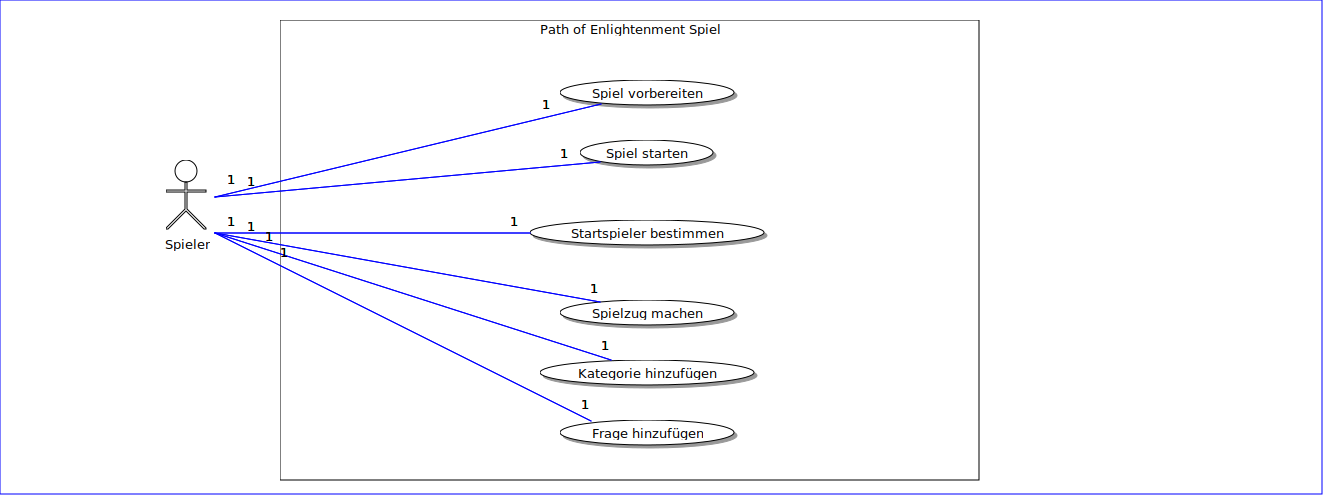
\includegraphics[width=0.9\textwidth]{UseCaseDiagram}
    \caption{Use Case Diagram für das Spiel}
  \end{center}
\end{figure}

\subsection{Use Case: Spiel vorbereiten}
\begin{labeling}[:]{Vorbedingungen}
\item [Akteure] Spieler
\item [Priorität] Wichtig
\item [Beschreibung] Die Spieler wählen aus den vorhandenen Kategorien 4 aus. Die Fragen jeder Kategorie werden gemischt. Jeder Spieler wählt eine Farbe für sich aus.
\item [Vorbedingungen] Es existieren mindestens 4 Kategorien
\item [Offene Punkte] Was wird gemacht, wenn weniger als 4 Kategorien existieren.
\end{labeling}

\subsection{Use Case: Startspieler bestimmen}
\begin{labeling}[:]{Vorbedingungen}
\item [Akteure] Spieler
\item [Priorität] Essentiell
\item [Beschreibung] Die Spieler würfeln der Reihe nach einmal mit einem Würfel. Der Spieler, dessen Wurf die höchste Augenzahl aufweist, darf beginnen. Sollten mehrere Spieler die gleiche höchste Augenzahl gewürfelt haben, so müssen nur diese erneut untereinander auswürfeln, wer beginnt. Dies wird so lange gemacht, bis ein Spieler eindeutig als Startspieler ausgemacht ist.
\item [Vorbedingungen] Spiel gestartet
\item [Offene Punkte]
\end{labeling}

\subsection{Use Case: Spielzug machen}
\begin{labeling}[:]{Vorbedingungen}
\item [Akteure] Spieler
\item [Priorität] Essentiell
\item [Beschreibung] Hat ein Spieler alle 3 Wissensstreiter auf seinen Heimatfeldern, darf er in diesem Zug 3 Mal würfeln um einen Wissensstreiter ins Spiel zu bringen. Er bringt einen seiner Wissensstreiter ins Spiel, indem er eine 6 würfelt. Würfelt er innerhalb dieser 3 Würfe eine 6, so wird einer seiner Wissensstreiter auf dem Pfad des Wissens platziert (auf dem entsprechenden Feld mit der Spielerfarbe) und sein Zug ist beendet. Sollte der Spieler nach den 3 Würfen keine 6 gewürfelt haben, so wird der Zug beendet und der nächste Spieler nach dem Uhrzeigersinn ist an der Reihe. \\
Hat ein Spieler mindestens einen seiner Wissensstreiter auf dem Pfad des Wissens, so würfelt er nur ein Mal. Würfelt er eine 6 und hat noch einen Wissensstreiter auf einem Heimatfeld, so muss er diesen ins Spiel bringen.
\\
Andernfalls kann der Spieler einen seiner Wissensstreiter um die gewürfelte Augenzahl auf dem Pfad nach vorne setzen. Er darf jedoch keinen seiner Wissensstreiter auf ein Feld setzen, auf dem sich schon ein anderer Wissensstreiter von ihm befindet.
\\
Kommt einer der Wissensstreiter auf ein Feld, auf dem bereits ein Wissensstreiter eines anderes Spieler steht, so beginnt eine \textbf{Fragerunde} mit diesem Mitspieler. Dies gilt auch dann, wenn ein Spieler einen seiner Wissensstreiter gerade erst von seinen Heimatfeldern auf den Pfad bringt und sein Startfeld auf dem Pfad durch einen anderen Spieler belegt ist.
\item [Vorbedingungen] Vorheriger Spielzug ist beendet worden. Bei erstem Spielzug: Startspieler bestimmt.
\item [Offene Punkte]
\end{labeling}

\subsection{Use Case: Fragerunde}
\begin{labeling}[:]{Vorbedingungen}
\item [Akteure] Spieler, Gegenspieler
\item [Priorität] Essentiell
\item [Beschreibung] Der Spieler stellt seinem Mitspieler (auch Geprüfter genannt) eine Frage aus einer der 4 Kategorien. Kann der Geprüfte die Frage beantworten, so kann dieser seinen Wissensstandanzeiger für die gewählte Kategorie auf die nächst höhere Stufe setzen. Ist die höchste Stufe bereits erreicht worden, so kann ein Wissensstandanzeiger in einer anderen Kategorie (die von dem Geprüften bestimmt wird) erhöht werden. Im Anschluss wird der Wissensstreiter des Geprüften auf dessen Startfeld gesetzt. Befindet sich dort bereits ein Wissensstreiter des selben Spielers, so wandert der Wissensstreiter auf eines der Heimatfelder.
\\
Sollte der Geprüfte die Frage jedoch nicht korrekt beantworten können, wird der Wissensstandanzeiger eine Stufe herabgesetzt und der Wissensstreiter landet direkt auf einem der Heimatfelder. Im Anschluss muss der Fragestellende die selbe Frage beantworten. Wenn er sie richtig beantwortet, bleibt seine Spielfigur auf dem Feld stehen und ansonsten gelten die selben Regeln, wie bei dem Geprüften. \\

Hat nach dem Zug ein Spieler alle Wissensstandanzeiger auf der höchsten Stufe, so gewinnt dieser das Spiel und das Spiel ist beendet.
\item [Vorbedingungen]
\item [Offene Punkte]
\end{labeling}

\newpage{}
\subsection{Use Case: Kategorie hinzufügen}
\begin{labeling}[:]{Vorbedingungen}
\item [Akteure] Spieler
\item [Priorität] Unwichtig
\item [Beschreibung] Der Spieler kann eine eigene Kategorie hinzufügen, der dann Fragen zugeordnet werden können.
\item [Vorbedingungen]
\item [Offene Punkte]
\end{labeling}

\subsection{Use Case: Frage hinzufügen}
\begin{labeling}[:]{Vorbedingungen}
\item [Akteure] Spieler
\item [Priorität] Unwichtig
\item [Beschreibung] Der Spieler kann eine Frage erstellen und mit einer Antwort versehen. Dann wird diese Frage einer Kategorie zugeordnet.
\item [Vorbedingungen] Kategorie vorhanden
\item [Offene Punkte]
\end{labeling}

\section{Begründung für die Priorisierung}\label{sec:begruendung-prio}
Die letzten beiden Punkte wurden als \texttt{unwichtig} eingestuft, da diese das Spielerlebnis zwar verbessern und personalisieren würden, jedoch ein Spiel ohne diese Funktionalität voll spielbar ist.\\
Das Spiel kommt nicht ohne die als \texttt{essentiell} gekennzeichneten Use Cases aus, da es ohne diese unspielbar ist. Ohne den Use Case \emph{Fragerunde} zum Beispiel, würde das Spiel keinen Gewinner und damit auch kein Ende finden.\\
Die Spielvorbereitung ist wichtig, da hierüber das Spielgeschehen maßgeblich gesteuert wird, also wie viele Spieler, mit welchen Kategorien spielen, aber sind nicht essentiell, da man hier auch mit festen Werten ein spielbares Spiel entwickeln könnte, was jedoch wenig Freude bereiten würde.

\section{Erste Iteration}
Für die erste Iteration werden lediglich die als \texttt{essentiell} priorisierten Use Cases implementiert. Dies sind die Folgenden

\begin{enumerate}
\item Startspieler bestimmen
\item Spielzug machen
\item Fragerunde
\end{enumerate}

Die Begründung für die Auswahl liegt in der Gewichtung, siehe hierzu \ref{sec:begruendung-prio}
